\thispagestyle{empty}

\begin{tikzpicture}[remember picture,overlay]
\node [opacity=1] at (current page.center) {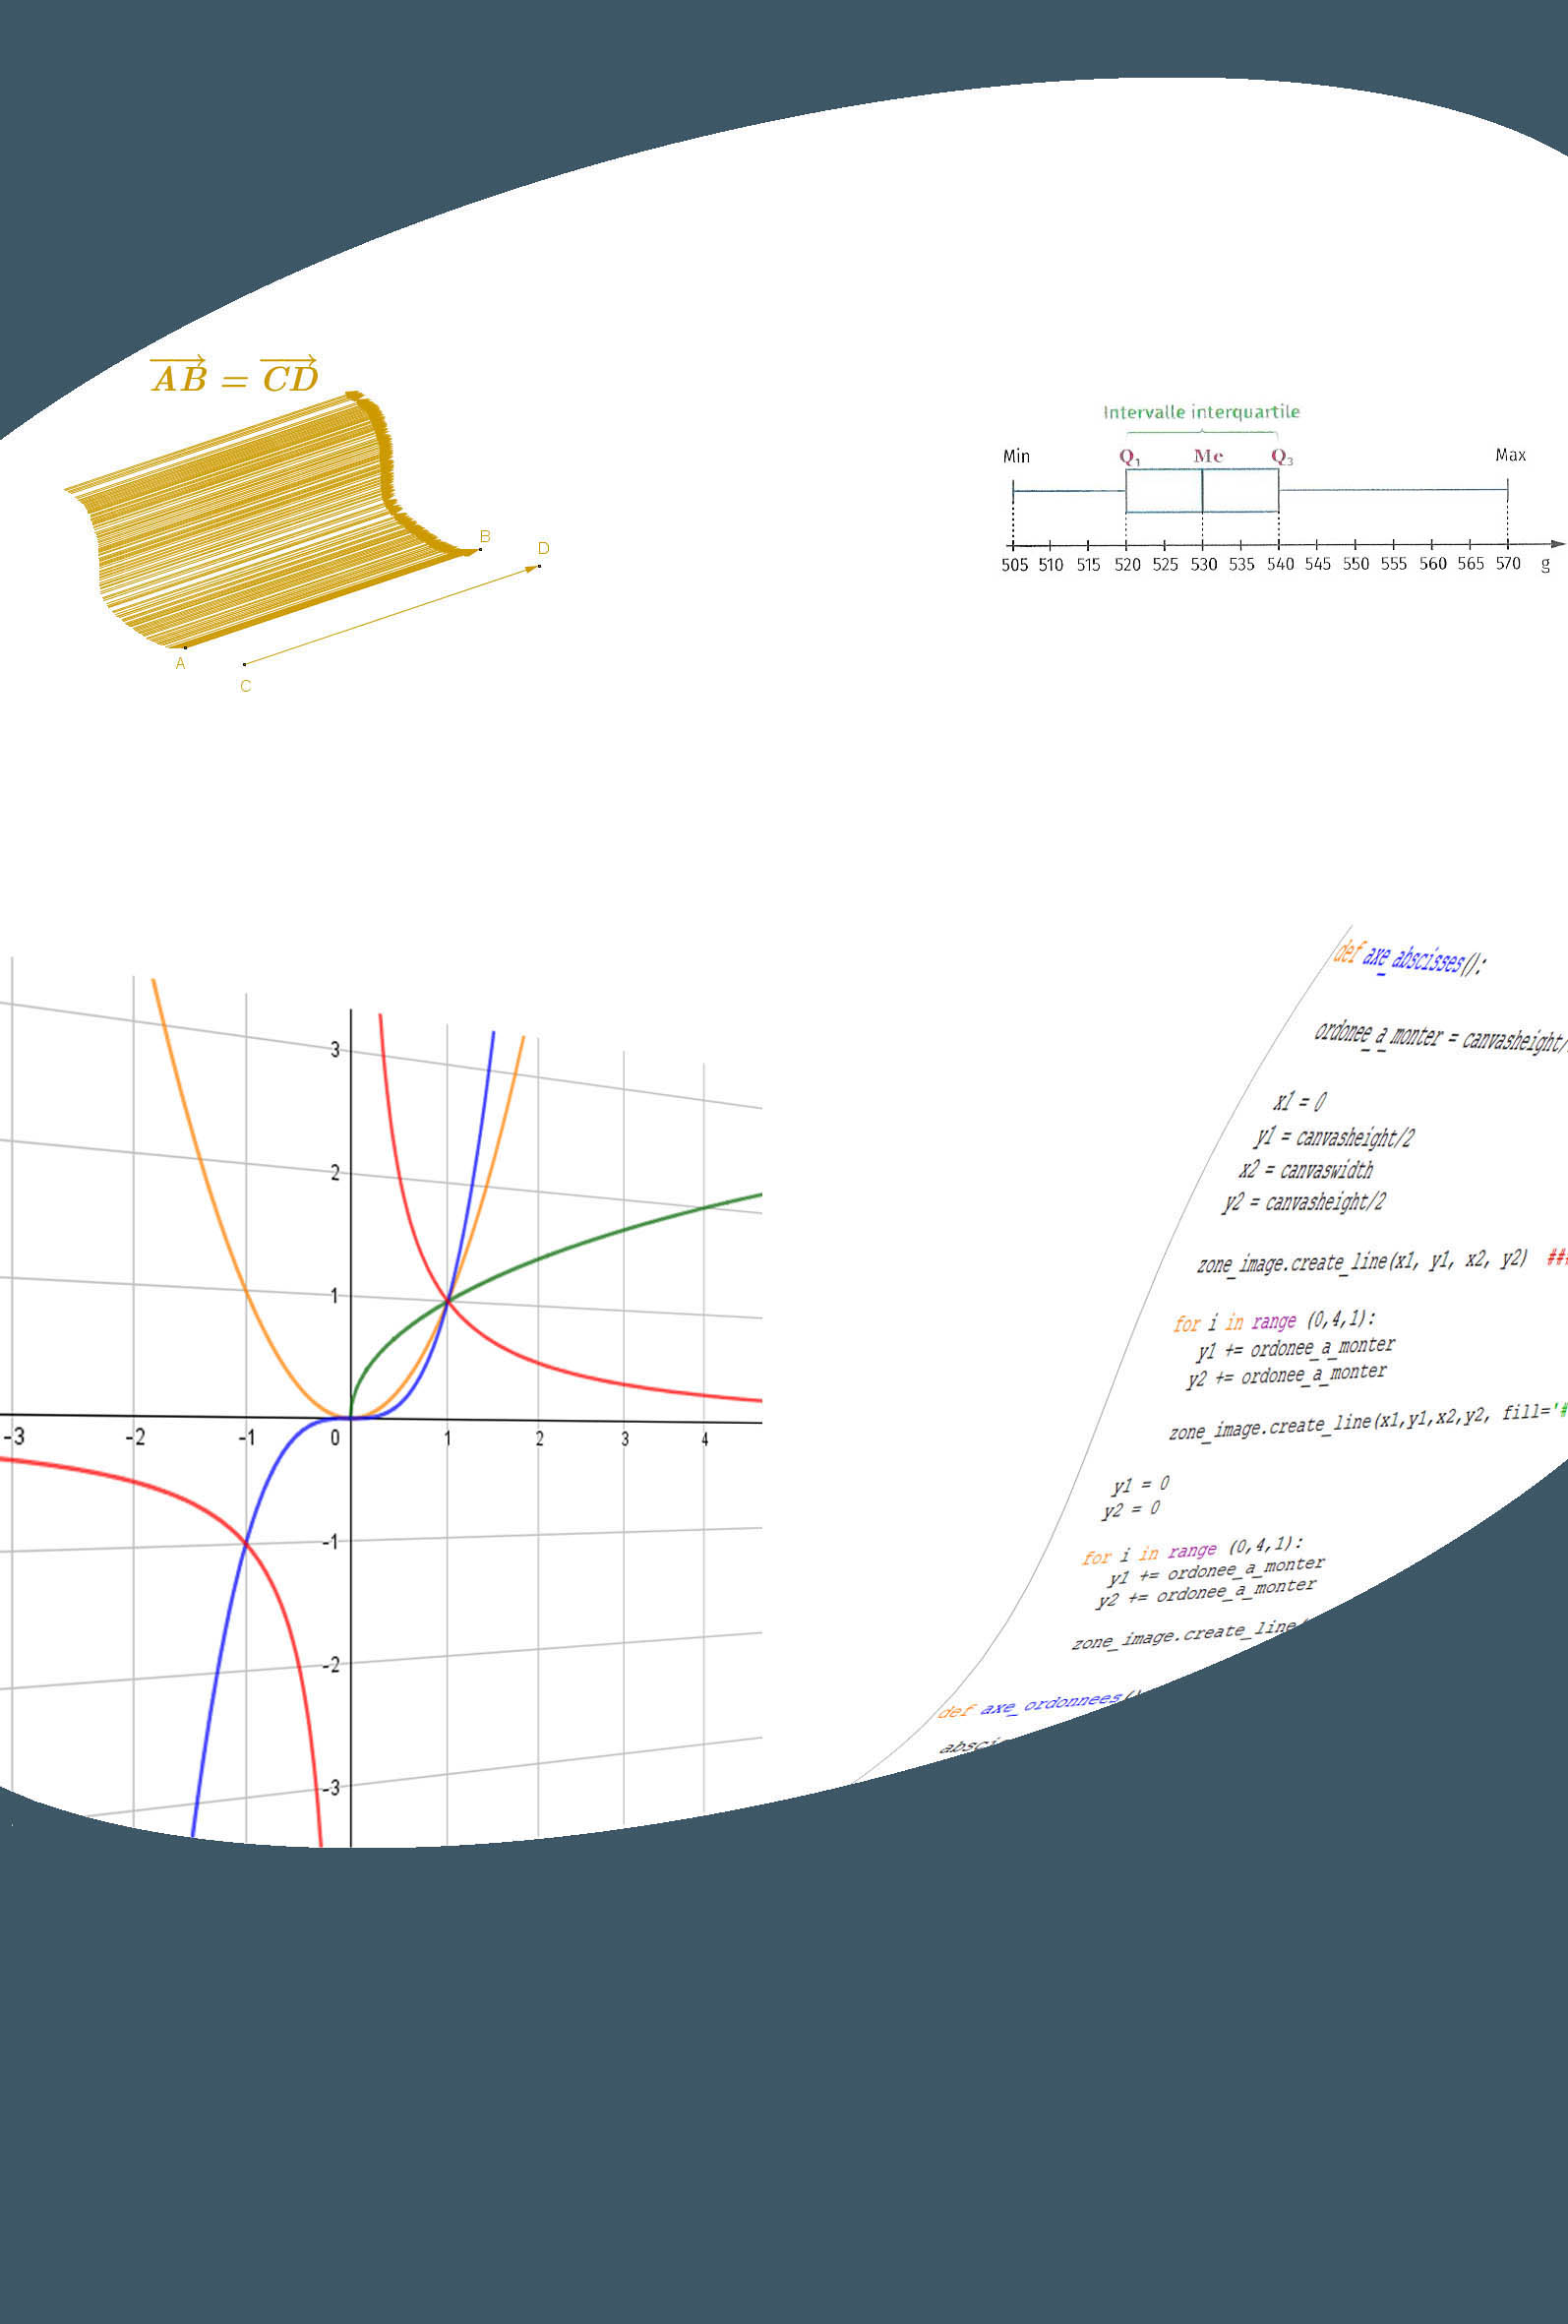
\includegraphics[width=21.7cm]{couverture.jpg} } ;
\end{tikzpicture}

\vspace{0.5cm}
\begin{center}
     {\color{bleu3} \textsc{\LARGE Lycée Français Gustave Flaubert}\\
    \vspace{0.5cm}
    \textsc{\Large La Marsa - TUNISIE}\\
 }
              \vspace{4.5cm}
              

     \begin{center}
        \textcolor{bleu3}{ {\fontsize{50}{50}\selectfont \bfseries {\sffamily {MATHÉMATIQUES}}} \\
          \vspace{2cm}
          \textbf{{\fontsize{30}{30}\selectfont {\sffamily Seconde}}}\\
             }
     \end{center}


 



 \vspace{6cm}  
 
    % Author and supervisor
    \begin{minipage}{0.4\textwidth}
      \begin{center} 

     {\color{bleu3}       \large{\textsc{ }}}
      \end{center}
    \end{minipage}
     
 \vfill
 \vspace{3cm} 
 
 
    % Bottom of the page
    {\large \textcolor{white}{Programme 2019}}\\
    
    {\large \textcolor{white}{Ce document est construit pour faciliter l'appréhension des notions par mes élèves. Il rassemble la majeure partie de ces notions abordées durant leur année de Seconde. \\ Ce fascicule est fortement inspiré du livre scolaire.}}
  \end{center}   


\newpage


  \tableofcontents 